\section{Monte Carlo model of Deep Exclusive $\pi^{-}$ Production from the
  Neutron in $^{3}$He }

The Monte Carlo studies needed for this proposal require a reaction
model for an experimentally unexplored region of kinematics, at higher
values of $Q^2$, $-t$ and $W$ than covered by existing data.  This appendix
describes the model and the constraints used.

\subsection{Definition of the Cross Section and Single-Spin Asymmetries}

The differential cross section for exclusive $\pi$ production from the nucleon
can be written as
\begin{equation}
  \frac{d^{5} \sigma}{dE' d\Omega_{e'} d\Omega_{\pi}} = \Gamma_{V} \frac{d{^2}
  \sigma}{d\Omega_{\pi}}.
\end{equation}
The virtual photon flux factor $\Gamma_{V}$ is defined as
\begin{equation}
  \Gamma_v=\frac{\alpha}{2\pi^2} \frac{E'}{E} \frac{K}{Q^2}\frac{1}{1-\epsilon},
\end{equation}
where $\alpha$ is the fine structure constant, $K$ is the energy of real photon
equal to the photon energy required to create a system with invariant mass
equal to $W$ and $\epsilon$ is the polarization of the virtual photon.
\begin{equation}
  K=(W^2-M_p^2)/(2 M_p)
\end{equation}
\begin{equation}
  \epsilon=\left(1+\frac{2 |\mathbf{q}|^2}{Q^2} \tan^2\frac{\theta_{e}}{2}
  \right)^{-1},
\end{equation}
where $\theta_{e}$ is the scattering angle of scattered electron.

The two-fold differential cross section $\frac{d{^2} \sigma}{d\Omega_{\pi}}$ in
the lab frame can be expressed in terms of the invariant cross section in
centre of mass frame of the photon and nucleon,
\begin{equation}
  \frac{d^2 \sigma}{d\Omega_\pi}= J \frac{d^2 \sigma}{dt d\phi},
\end{equation}
where $J$ is the Jacobian of transformation of coordinates from lab
$\Omega_{\pi}$ to $t$ and $\phi$ (CM). 

Following Ref.~\cite{hermes-thesis}, we consider separately the unpolarized and
polarized target contributions to the invariant photon nucleon cross section,
\begin{equation}
  d\sigma = d\sigma_{UU} + d\sigma_{UT}.
  \label{eqn:cross-1}
\end{equation}

In the one-photon exchange approximation, the unpolarized nucleon 
cross section for $n(e,e^{\prime}\pi^{-})p$
can be expressed in four terms. Two terms correspond
to the polarization states of the virtual photon (L and T) and two states
correspond to the interference of polarization states (LT and TT),
\begin{equation}
  d\sigma_{UU} =  \epsilon  \frac{d\sigma_{\mathrm{L}}}{dt}
  + \frac{d\sigma_{\mathrm{T}}}{dt} + 
  \sqrt{2\epsilon (\epsilon +1)} \frac{d\sigma_{\mathrm{LT}}}{dt} \cos{\phi}
  + \epsilon  \frac{d\sigma_{\mathrm{TT}}}{dt} \cos{2 \phi},
  \label{eqn:cross-2}
\end{equation}
where $\phi$ is the angle between lepton plane and hadron plane
(Fig.~\ref{fig:planes}). 
The first two terms of Eqn.~\ref{eqn:cross-2} correspond to the
polarization states of the virtual photon (L and T) and last two terms
correspond to the interference of polarization states (LT and TT).  $\epsilon$
is the ratio of longitudinal to transverse virtual-photon fluxes
\begin{equation}
  \epsilon=\left(1+\frac{2
  |\mathbf{q}|^2}{Q^2} \tan^2\frac{\theta_{e}}{2} \right)^{-1}.
\end{equation}
The constraints used to parameterize $d\sigma_{UU}$ are described in
Sec.~\ref{sec:model}.

The additional contribution when the target nucleon is transversely polarized
can be parameterized \cite{Di05,hermes-thesis} as
\begin{equation}
  d\sigma_{UT} = -\frac{P_{T}}{\sqrt{1 - \sin^{2}{\theta} \sin^{2}{\phi_{S}} }
  } \sum_{k=1}^{6} \sin{ (\mu\phi + \lambda\phi_{S})
  } \Sigma_{k},
\label{eqn:cross-3}
\end{equation}
where $\phi_{S}$ is angle between the target polarization and lepton planes
(Fig.~\ref{fig:planes}) and the $\Sigma_{k}$ are given by
\begin{equation}
  \Sigma_{k} = A_{UT}^{\sin{( \mu\phi+\lambda\phi_{S})_{k}}} \times
  d\sigma_{UU}(\phi).
  \label{eqn:sigmas}
\end{equation}
The $\sin{( \mu\phi+\lambda\phi_{S})_{k}}$ are the six azimuthal modulations
\begin{tabular}{|r|l|}
\hline
k & $\sin{(\mu\phi + \lambda\phi_{S})_{k}}$ \\
\hline
1 & $\sin{(\phi - \phi_{S})}$ \\ 
\hline
2 & $\sin{(\phi + \phi_{S})}$ \\ 
\hline
3 & $\sin{(\phi_{S})}$ \\ 
\hline
4 & $\sin{(2\phi - \phi_{S})}$ \\ 
\hline
5 & $\sin{(3\phi - \phi_{S})}$ \\ 
\hline
6 & $\sin{(2\phi + \phi_{S})}$ \\ 
\hline
\end{tabular}
.\\
For $k=1-5$, the $A_{UT}^{\sin{( \mu\phi+\lambda\phi_{S})_{k}}}$ used here are
the asymmetries calculated for us by Sergey Goloskokov and Peter Kroll
\cite{GoPC} for SoLID-DEMP kinematics (see Fig.~\ref{fig:gk16}).  The asymmetry
for $k=6$ is a fit of HERMES data \cite{hermes-thesis}.  Further details are
provided in Sec.~\ref{sec:sixparametrizations}.

\subsection{Cross Section Model for Higher $Q^2$ Kinematics
\label{sec:model}}

\subsubsection{Constraints}

All of the following data were used as constraints on the parameterizations
used in this model.
\begin{itemize}
\item
From Hall C, precise $L/T$ separated experimental data of exclusive
electroproduction of $\pi^{-}$ on $^2$H are available up to $Q^2=2.57$ GeV$^2$,
$-t=0.350$ GeV$^2$ and $W=2.168$ GeV \cite{gmhuber-2}.
\item
Also from Hall C, precise $L/T$ separated experimental data of exclusive
electroproduction of $\pi^{+}$ on $^1$H are available up to $Q^2=2.703$
GeV$^2$, $-t=0.365$ GeV$^2$ and $W=2.127$ GeV \cite{Fpi2}, and separated
$\sigma_{L}$ and $\sigma_{T}$ are measured up to $Q^2=4.703$ GeV$^2$ and
$W=2.2$ GeV \cite{hallc-1} and \cite{hallc-2}.
\item
CLAS experiment E99-105 measured the unseparated exclusive $\pi^+$ cross
section from $^1$H at $Q^2$ up to $4.35$ GeV$^2$ and $-t$ up to $4.5$ GeV$^2$
\cite{park}.
\item
The HERMES collaboration measured the unseparated cross section for $Q^2$=3.44
GeV$^2$ and 5.4 GeV$^2$ \cite{hermes} at $W$=4 GeV.
\end{itemize}

An additional constraint in our parameterization comes from the
Vrancx-Ryckebusch (VR) model \cite{vr}.  This is a Regge model with a
parametrization of the deep inelastic scattering amplitude added to improve the
description of $\sigma_{T}$.  The description of $\sigma_{L}$ in the model is
constrained by a fit to the Hall C $p(e,e'\pi^+)n$ data from
Ref.~\cite{gmhuber}.  The model provides a good description of exclusive
charged pion electroproduction above the resonance region.  It has been checked
for reliability against the Hall B and C data listed above, for $W>2$ GeV,
$Q^2$ from 0.35 to 4.98 GeV$^2$.  The model is believed to be reliable for
$-t\leq$0.5 GeV$^2$, but it overshoots the data for $-t>$0.5 GeV$^2$.

\begin{figure}[!hbt]
    \centering
%    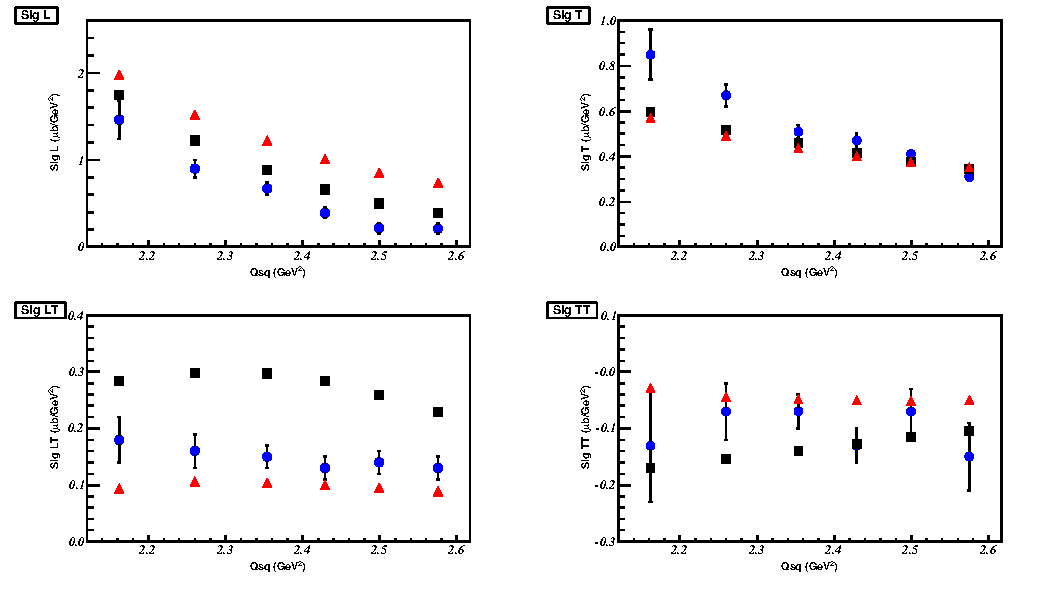
\includegraphics[width=6.0in,height=2.4in]{./figures/pimsigma_qsq.pdf}
    \includegraphics[width=6.0in,height=3.0in]{./figures/01.eps}
    \caption{ A comparison of last six points of table $v$ of \cite{gmhuber-2},
      the VR model, and our parametrization values vs. $Q^{2}$ for $\pi^{-}$
      electroproduction. Experimental data are shown in blue circles, VR model
      is shown in red triangles, and our parametrization is shown in black
      boxes. In each graph, the value of $-t$ is decreasing left to right from
      a maximum value 0.35 GeV$^2$ to 0.15 GeV$^2$. Value of $W$ also decreases
      left to Right from 2.2978 GeV to 2.1688 GeV.}
    \label{fig:expvrfit}
\end{figure}

\begin{figure}[!hbt]
    \centering
%    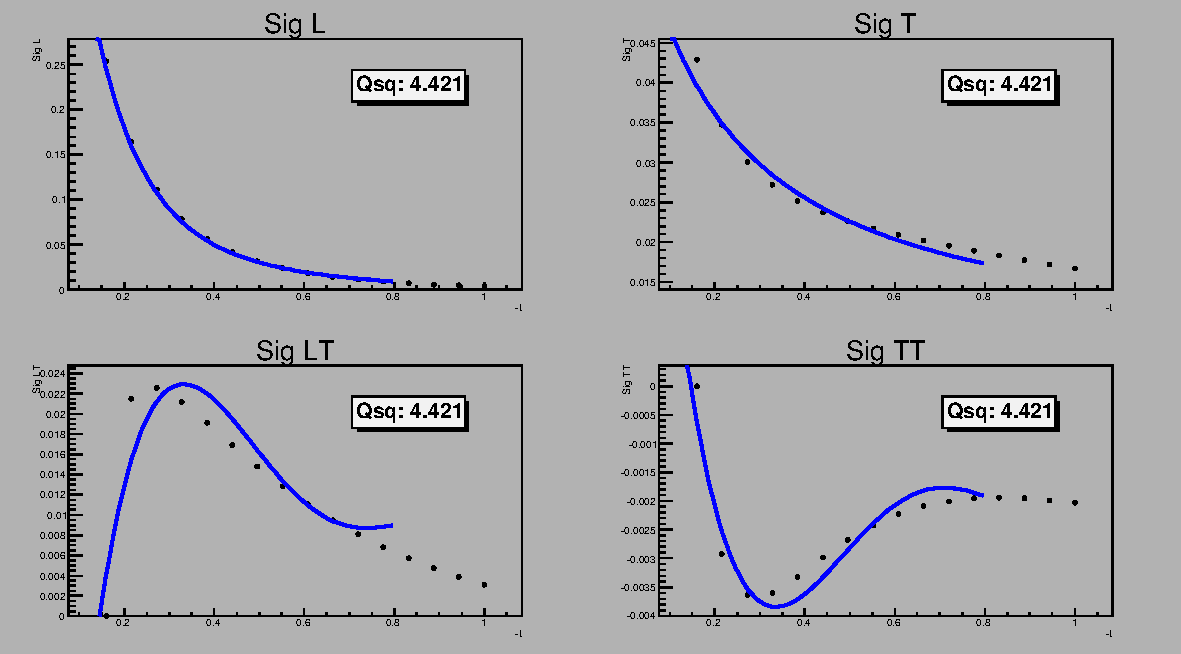
\includegraphics[width=6.0in,height=2.4in]{./figures/pimFit.pdf}
    \includegraphics[width=5.0in,height=2.4in]{./figures/02.eps}
    \caption{ A comparison of parametrized $\sigma_{L,T,LT,TT}$ and VR model
    values at $Q^2$ = 4.421 GeV$^2$ and $W = 3.0$ GeV.  Black points are VR
    model values and blue line is parametrized $\sigma_{L,T,LT,TT}$ given by
    equations $\ref{equation:l-fit}$ to $\ref{equation:tt-fit}$. }
    \label{fig:sigall}
\end{figure}

\subsubsection{Parametrization of $\sigma_{L}$, $\sigma_{T}$, $\sigma_{LT}$, 
$\&$ $\sigma_{TT}$
\label{sec:parametrization}}

For exclusive DEMP in SoLID, the kinematic region of interest for
parametrization of $\sigma_{L,T,LT,TT}$ is $Q^2$ from 4.0 GeV to 7.5 GeV$^2$,
$-t$ from 0 GeV$^2$ to 1.0 GeV$^2$, and we set $W=3.0$ GeV. After the
parametrization of $\sigma_{L,T,LT,TT}$ for $-t$ and $Q^2$, we used the same
$W$ dependence given by \cite{gmhuber}, which is $(W^2-M^2)^{-2}$ where $M$ is
the proton mass.  Our parametrization of all four cross sections is given in
equations $\ref{equation:l-fit}$ to $\ref{equation:tt-fit}$.

\begin{equation}
        \sigma_{L} = \exp{(P_1(Q^2) + |t| * P^{\prime}_1(Q^2))}
        + \exp{(P_2(Q^2) + |t| * P^{\prime}_2(Q^2))}
     \label{equation:l-fit}
\end{equation}

\begin{equation}
        \sigma_{T} = \frac{\exp{(P_1(Q^2) + |t| *
        P^{\prime}_1(Q^2))}}{P_{1}(|t|)}
     \label{equation:t-fit}
\end{equation}

\begin{equation}
        \sigma_{LT} = P_{5}(t(Q^2))
     \label{equation:lt-fit}
\end{equation}

\begin{equation}
        \sigma_{TT} = P_{5}(t(Q^2))       
     \label{equation:tt-fit}
\end{equation}

Here, the parameters $P_{i}$ are polynomial functions of $i^{th}$ order. Each
coefficient ($P_{i}$) of the fifth order equations $\ref{equation:lt-fit}$ and
$\ref{equation:tt-fit}$ is a further second order polynomial of $Q^2$. Deep
exclusive $\pi^{-}$ events are generated using a C++ code. The quality of
parametrization is checked by plotting the parametrization functions of
$\sigma_{L,T,LT,TT}$ versus the existing data and the VR model are shown in 
Figs. \ref{fig:expvrfit}, \ref{fig:sigall}.

{\bf There is no statement made that the cross section is calculated in the
  neutron rest frame from the `vertex' kinematic quantities, and then
  transformed to the lab frame.}

\subsection{Parametrization of the six Single-Spin Asymmetries
\label{sec:sixparametrizations}}

Six asymmetries of Eqn. \ref{eqn:sigmas} are calculated by Sergey 
Goloskokov and Peter Kroll for the SoLID DEMP kinematics of this proposal.

{\bf
Need to add a description of the fit to their calculations.  Also need to add
the parametrization of the sixth asymmetry from HERMES data.

The calculation of the components of $\sigma_{UT}$ from these asymmetries needs
to be described, including the transformation from the neutron rest frame to
the lab frame.
}

\begin{figure}[!hbt]
    \centering
    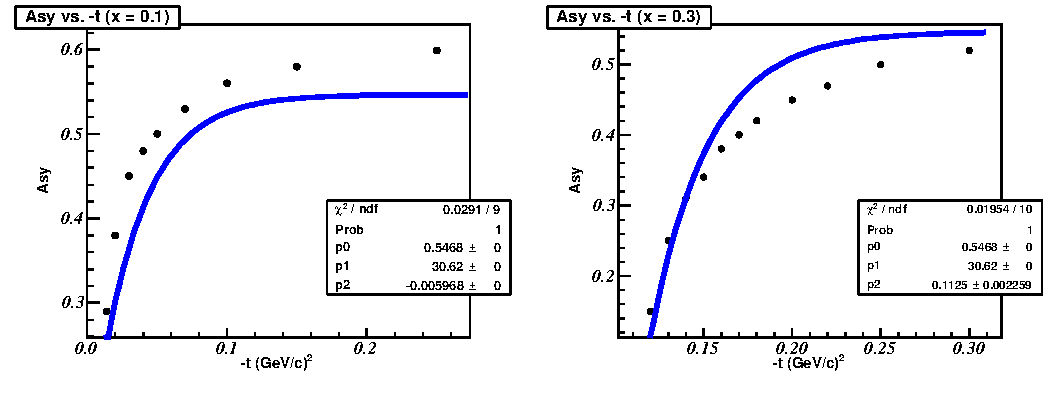
\includegraphics[width=6.0in,height=1.45in]{./figures/asym_3.pdf}
    \caption{ Parametrization of single spin asymmetry $\bf{A_{L}^{\perp}}$
      vs. $-t$ at $Q^2$ = 10 GeV$^2$ in left graph $x = 0.1$ and in right graph
      $x = 0.3$ where the points are from the model defined in \cite{Fr00} and
      blue line is our parametrization function.}
    \label{fig:asym-1}
\end{figure}

%It is shown in Ref. \cite{frankfurt} that the generalized parton distribution
%($\tilde{E}$) can be probed by measuring the single spin asymmetry$(SSA)$. The
%SSA is defined in equation $\ref{eqn:ssa}$, where $\beta$ is the angle
%between the transversely polarized target vector and the reaction plane, and
%$\sigma_{L}^{\pi^{-}}$ is the exclusive $\pi^{-}$ cross section for
%longitudinal virtual photons.  We parametrized the single spin asymmetry using
%the model of \cite{frankfurt} at $x=0.1$ and $x=0.3$. Our parametrization of
%$SSA$ is shown in Fig. $\ref{fig:asym-1}$ and equation
%$\ref{eqn:asy-fit}$ is the parameterized function of single spin
%asymmetry.
%
%\begin{equation}
%  \bf{A_{L}^{\perp}} =
%\frac{\int^{\pi}_{0}d\beta\frac{d\sigma_{L}^{\pi^{-}}}{d\beta} -
%\int^{2\pi}_{\pi}d\beta\frac{d\sigma_{L}^{\pi^{-}}}{d\beta} }
%{\int^{2\pi}_{0}d\beta\frac{d\sigma_{L}^{\pi^{-}}}{d\beta}}
%     \label{eqn:ssa}
%\end{equation}
%
%\begin{equation}
%        \bf{A_{L}^{\perp}} = \left\{
%        \begin{array}{rl}
%        A_{0} \left[ 1 - \exp^{ [ -\lambda \times ( t - t_{min} ) ] } \right] & \text{if } t \ge t_{min}, \\
%        0 &  \text{if } t < t_{min}.
%        \end{array} \right.
%     \label{eqn:asy-fit}
%\end{equation}

\subsection{Target Neutron Fermi Momentum 
\label{sec:fermimotion}}

\begin{figure}[!hbt]
    \centering
    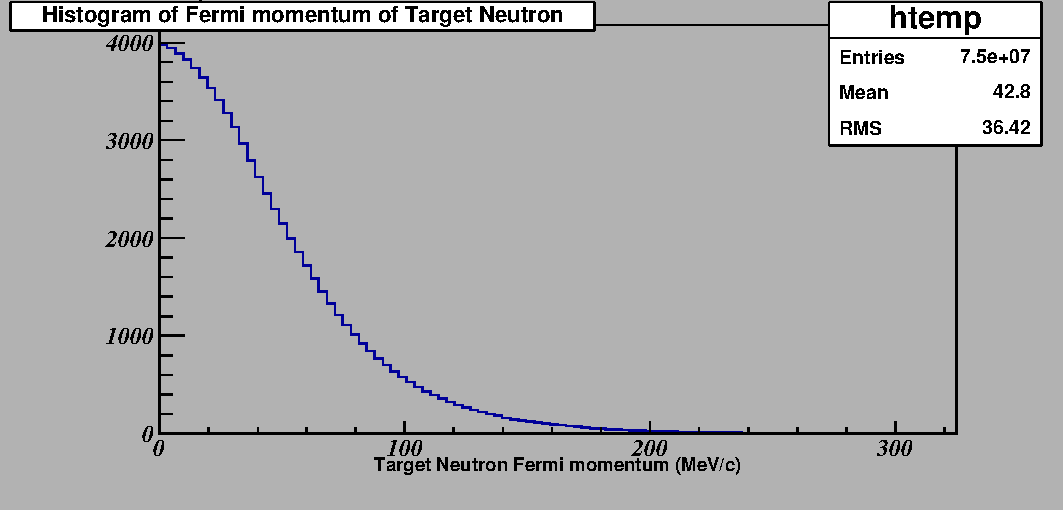
\includegraphics[width=4.0in,height=2.5in]{./figures/Fermi.pdf}
%    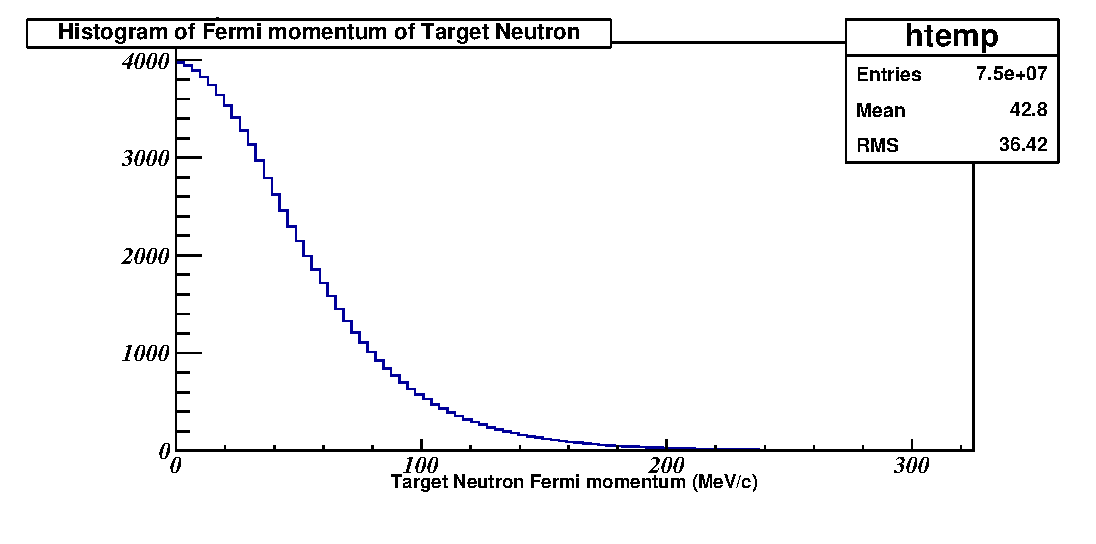
\includegraphics[width=4.0in,height=2.5in]{04.eps}
    \caption{Fermi momentum spectral function of a target nucleon in $^3$He
      generated according to the Argonne potential of Ref \cite{fermipaper}.
      The horizontal axis is nucleon momentum in MeV/c.}
    \label{fig:fermi}
\end{figure}

A histogram of the spectral function of $^3$He is shown in
Fig.~\ref{fig:fermi}, generated according to Ref.~\cite{fermipaper}. Neutron
momenta up to 300 MeV/c are generated according to this distribution, uniformly
distributed in spherical coordinates. The quasi-free collision between the
virtual photon and moving neutron is then transformed to the fixed neutron
frame, after which the parameterizations of Secs.~\ref{sec:parametrization},
\ref{sec:sixparametrizations} are applied. The outgoing particles are then
transformed back to the lab frame for tracking.

\subsection{Energy Loss and Multiple Scattering
\label{sec:energyloss}}

There is energy loss for the incoming electron $e$, and the three outgoing
particles: scattered electron $e^{\prime}$, $\pi^{-}$ and recoil proton $p$ by
bremsstrahlung and ionization.  The same code as given in SAMC (Hall A Single
Arm Monte Carlo) \cite{samc} is used.  This code is based on Sec. 33 (Passage
of articles through matter) of the Review of Particle Physics by the Particle
Data Group \cite{pdg}.

Incoming electron and three out going particles are deflected small angles by
multiple scattering in the target, target window and in the air. This small
deflection in the polar angle theta $\theta$ is calculated according to
Subsection 33.3 (Multiple scattering through small angles) of the Review of Particle
Physics by the Particle Data Group \cite{pdg}.

The incoming electron loses energy by bremsstrahlung and ionization, and
suffers multiple scattering, in the target and in the target window.  Both of
these processes and the choice of neutron Fermi momentum are applied before the
cross section terms $\sigma_{uu}$ and $\sigma_{UT}$ are calculated from the
`vertex' kinematic quantities.

The scattered electron, pion and proton lose energy by bremsstrahlung and
ionization, and suffer multiple scattering, in the target, target window and in
the air.  The energy and momentum of these particles are corrected according to
these processes prior to particle tracking.

\subsection{Final State Interactions
\label{sec:fsi}}

A separate version of the model was made in which the outgoing $\pi^-$ suffers
$\pi N$ final state interactions (FSI) with one of the recoil $p$ in the
residual nucleus.

The scattering of $\pi^-$ by protons involves both the $T=1/2$ and $T=3/2$
isospin states.  We model the $\pi^- p$ scattering via the empirical phase
shift analysis of Rowe, Solomon and Landau \cite{rowe}.  In this case,
the amplitude for the scattering of a spin-zero particle by a particle of
spin-$\frac{1}{2}$ is described for each isospin channel by a set of partial
wave amplitudes $f^{(+)}_{\ell}$, $f^{(-)}_{\ell}$ for the
$j=\ell\pm\frac{1}{2}$ states.  In terms of phase shifts, $f^{(+)}_{\ell}$ is
\begin{equation}
f^{(+)}_{\ell}\equiv\frac{1}{2ik}(e^{2i\delta^+_{\ell}} -1)
\end{equation}
with a similar expression for $f^{(-)}_{\ell}$.  The phase shift
$\delta^+_{\ell}$ will be complex if there is any inelasticity, which will
occur for example for the reactions
\begin{equation}
\begin{split}
\pi^- + p &\rightarrow \pi^+ \pi^- p \\
          &\rightarrow \pi^0 \pi^0 n \\
          &\rightarrow \pi^- \pi^0 p. \\
\end{split}
\end{equation}
The differential cross-section is written in terms of these phase shifts as
\begin{equation}
\frac{d\sigma}{d\Omega}=\biggl[
\biggl| \frac{1}{k}\sum_{\ell}[(\ell +1) 
f^{(+)}_{\ell} +\ell f^{(-)}_{\ell}] P_{\ell}(\cos\theta)\biggr|^2 +
\biggl| \frac{i}{k}\sum_{\ell}[f^{(+)}_{\ell} -f^{(-)}_{\ell}]\sin\theta 
 \frac{d P_{\ell}(\cos\theta)}{d\cos\theta}\biggr|^2
\biggr].
\label{eqn:piN}
\end{equation}

$\pi N$ phase shifts have been determined experimentally from near threshold up
to several GeV.  The dominant phase shifts for the $L_{2T,2J}$ states:
S$_{11}$, S$_{31}$, P$_{11}$, P$_{13}$, P$_{31}$, P$_{33}$ are very accurately
known for centre of mass momenta up to 350 MeV/c.  The phase shift
parameterizations used in our model are dominated by the $\Delta(1232)$ and
$N^*(1440)$ resonances.  For further information, please see
Ref.~\cite{ericson}.

In our implementation of the FSI process, the Fermi momentum of one of the
recoil protons was chosen according to Sec.~\ref{sec:fermimotion} and collided
with the outgoing $\pi^-$ in their mutual centre of mass frame.  Outgoing
$\pi^-$ $N$ were randomly generated, and the events
weighted according to the differential cross setions of Eqn.~\ref{eqn:piN}.
Events were generated for both the FSI and non-FSI versions of the
model and the results compared, as described in the main text.






